%----------------------------------------------------------------------------------
% Exemplo do uso da classe tcc.cls. Veja o arquivo .cls
% para mais detalhes e instruções.
%----------------------------------------------------------------------------------

% PARA PREENCHIMENTO DO REVISOR:
% CHECKLIST
% [ ] Introduction: check the introduction 
    % [ ] Avoid jargon: Do you avoid jargon that is only explain in the rest of the text?
    % [ ] Clarity: Can anyone from computer science read the introduction and understand what's the objective?
    % [ ] Does it clearly describe the problem?
    % [ ] Does the introduction clearly state the contributions?

\sigla{COLREGS}{Collision Regulations at Sea}
\sigla{LSA}{Laboratório de Sistemas Autônomos}
\sigla{USV}{Unmanned Surface Vehicle}
\sigla{VO}{Velocity Obstacles}

\chapter{Introdução}\label{chap1:intro}
    É significativo o número de importantes atividades aquáticas realizadas por seres humanos utilizando embarcações~\cite{LIU201671}. Porém, tais tarefas podem ser longas e entediantes, dificultando a constância de foco que deve ser mantida durante a execução~\cite{JURAK2020}. A distração pode levar a sérias consequências em um cenário onde há diversas embarcações na mesma área. Investigações mostram que o fator humano~\cite{HUANG2020451}, junto com o descumprimento de regras marítimas de evasão de colisão (COLREGS - do inglês \textit{"COLlision REGulations at Sea"})~\cite{JURAK2020}, são as principais causas de acidentes envolvendo embarcações.
    Visando eliminar o fator humano e possibilitando a realização de tarefas longas, perigosas e com maior precisão, estudos sobre veículos de superfície não tripulados (USV - do inglês \textit{"Unmanned Surface Vehicle"}) vêm ganhando atenção~\cite{LIU201671}.
    
    USV é um veículo que se move de forma autônoma através de um sistema embarcado ou distribuído~\cite{SONG2018351}. Com o desenvolvimento de USVs e sua atuação em meios comuns a outras embarcações (TS - do inglês \textit{"Target Ship"}), tripuladas ou não tripuladas, é inevitavel que situações de colisão aconteçam. O principal desafio, atualmente, no desenvolvimento de um USV consiste em torná-lo capaz de evitar colisões. Contudo, apenas evitar colisão não é suficiente, é preciso que o USV se movimente de acordo com as mesmas regras aplicadas aos seres humanos, ou seja, de acordo com as COLREGS~\cite{JURAK2020}. É importante que essa diretiva seja considerada no desenvolvimento de USVs, visto que em um cenário de colisão eminente entre um USV e um TS, a outra embarcação deve ser capaz de identificar a movimentação do USV como uma evasão da colisão~\cite{KUWATA2014110}.
    
    Apesar de importantes, as COLREGS são normas destinadas à compreensão de seres humanos e deixam margens para interpretação, fazendo com que uma COLREGS possa ser aplicável, ou não, dependendo de cada caso~\cite{KUWATA2014110}. Consequentemente, em um cenário onde múltiplas embarcações possuem trajetos que se cruzam em algum ponto, é desejável que o sistema de um USV seja capaz de prever se em algum momento haverá risco de colisão com alguma embarcação próxima. Nesse sentido, um método muito utilizado para verificar risco de colisão é o CPA (do inglês \textit{"Closest Point of Approach"}), onde é analisada a distância entre as embarcações no momento em que elas estarão mais próximas~\cite{HUANG2019142}. Se essa distância não for considerada segura, um risco de colisão é detectado e um procedimento de evasão deverá ser iniciado.
    
    Com base nas informações apresentadas, o presente trabalho visa desenvolver uma aplicação capaz de detectar o CPA e identificar qual encontro previsto na COLREGS é aplicável. Ademais, será realizada a integração em um sistema para USV já existente, para que seja possível realizar simulações e analisar se o comportamento resultante está de acordo com o esperado. O presente documento está estruturado da seguinte forma: no capítulo \ref{chap1:intro}, além das informações já apresentadas, o trabalho proposto será aprofundado na sessão \ref{subchap1:trab_prop}, e as contribuições serão evidenciadas na sessão \ref{subchap1:contrib}. O capítulo \ref{chap2:fund_teo} contém uma revisão teórica apresentando maiores detalhes a respeito de USV na sessão \ref{subchap2:USV}, COLREGS na sessão \ref{subchap2:colregs} e prevenção de colisão na sessão \ref{subchap2:prev_col}.
    
    \section{Trabalho Proposto}\label{subchap1:trab_prop}
        Motivado pela vontade de experienciar o processo científico, este trabalho se propõe a realizar uma breve revisão da literatura sobre evasão de colisão aplicado a USV, identificando as técnicas utilizadas atualmente. Como resultado do estudo, será desenvolvida uma aplicação que seja capaz de detectar o CPA entre um USV e um TS prevendo qual regra da COLREGS será aplicável ao encontro. Por fim, para que seja possível analisar o comportamento resultante da implementação, a aplicação será integrada a um sistema para USV já existente, desenvolvido por Jurak~\cite{JURAK2020}.
        
        Jurak~\cite{JURAK2020} desenvolveu um sistema de código aberto para evasão de colisão com respeito à COLREGs para veículos não-tripulados que navegam na superfície da água. Seu trabalho foi realizado utilizando o framework de desenvolvimento ROS (do inglês \textit{"Robot Operating System"}) e utilizou o simulador USV\_sim para realizar seus testes e obter seus resultado. Com base nisso, este trabalho será desenvolvido com base nos mesmos paradigmas ROS para que haja compatibilidade com o sistema de Jurak~\cite{JURAK2020}, possibilitando a integração. Consequentemente, o mesmo simulador será utilizado para realização dos testes.
        
    \section{Contribuições}\label{subchap1:contrib}
        A primeira contribuição deste trabalho é capacitar o sistema desenvolvido por Jurak~\cite{JURAK2020} a calcular o CPA, para que possa ser utilizado nos barcos-robôs pertencentes ao Laboratório de Sistemas Autônomos da PUCRS. Além disso, a maioria dos sistemas desenvolvidos para USVs ou são resguardados por patentes, ou então possuem acesso restrito àqueles que não participaram de seu desenvolvimento.~\cite{JURAK2020} Sendo assim, este trabalho visa contribuir à comunidade de desenvolvedores mantendo o que for desenvolvido em código aberto.
        
        A segunda contribuição, em decorrência da primeira, será identificar encontros em que as COLREGS não são aplicáveis. Kuwata \etal nos mostra, através da Figura
        
        % Contribuições previamente listadas, serão melhor trabalhadas em um texto apropriado.
        
        % \begin{itemize}
        %     \item Adicionar CPA
        %     \item Com o CPA será possível identificar situações onde a COLREGS pode ser aplicável ou não
        %     \item Com a capacidade de identificar colisões com VO, há a possibilidade de aprimorar o sistema para suportar encontro com múltiplas embarcações. Só teria que ver como ficaria a sincronia entre o VO e o método ATC (presente no sistema atualmente).
        % \end{itemize}
        
        \begin{figure}
            \centering
            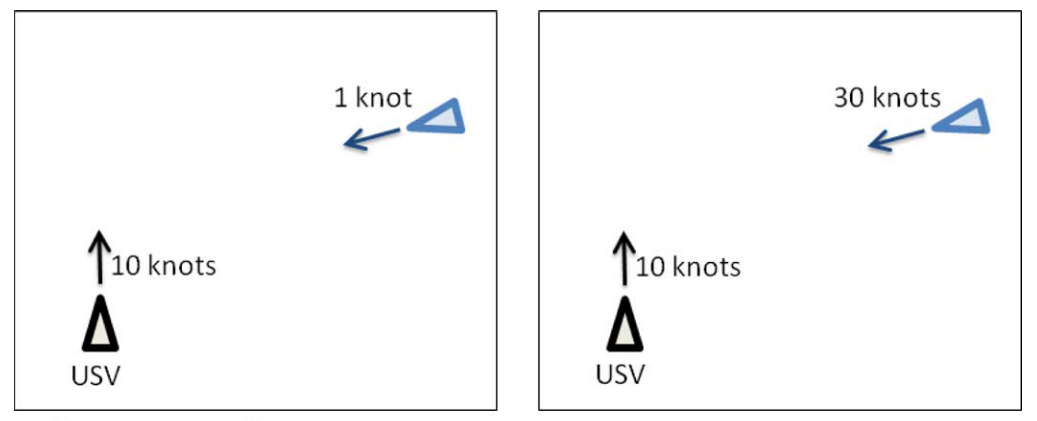
\includegraphics[width=\textwidth]{fig/colregs_situation_not_applied.png}
            \caption{Caption}
            \label{fig:colregs_na}
        \end{figure}